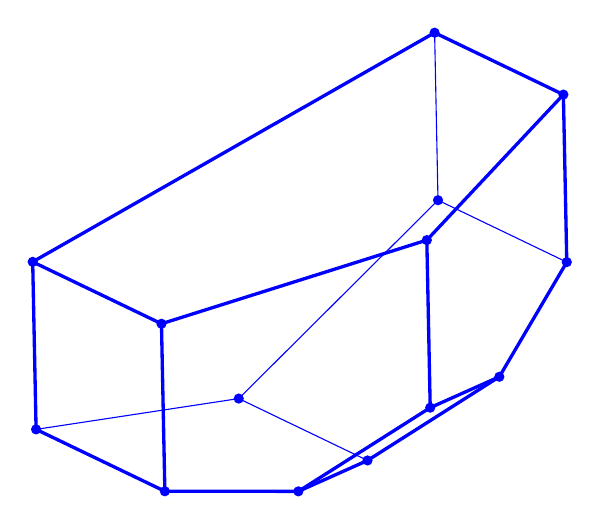
\begin{tikzpicture}%
	[x={(0.681462cm, -0.327528cm)},
	y={(0.731633cm, 0.326817cm)},
	z={(-0.017949cm, 0.886519cm)},
	scale=.60000,
	back/.style={color=blue, thin},
	edge/.style={color=blue, very thick, },
	facet/.style={fill=blue,fill opacity=0.00000},
	vertex/.style={inner sep=1pt,circle,draw=blue,fill=blue,thick}]
%
%
%% This TikZ-picture was produce with Sagemath version 9.5
%% with the command: ._tikz_3d_in_3d and parameters:
%% view = [-764, -346, -545]
%% angle = 76.39
%% scale = 1
%% edge_color = blue
%% facet_color = blue
%% opacity = 0.5
%% vertex_color = blue
%% axis = False

%% Coordinate of the vertices:
%%
\coordinate (-1.00000, -4.00000, -3.00000) at (-1.00000, -4.00000, -3.00000);
\coordinate (1.00000, 0.00000, -3.00000) at (1.00000, 0.00000, -3.00000);
\coordinate (3.00000, 4.00000, 1.00000) at (3.00000, 4.00000, 1.00000);
\coordinate (3.00000, 2.00000, -1.00000) at (3.00000, 2.00000, -1.00000);
\coordinate (3.00000, 0.00000, -1.00000) at (3.00000, 0.00000, -1.00000);
\coordinate (1.00000, -2.00000, -3.00000) at (1.00000, -2.00000, -3.00000);
\coordinate (3.00000, 4.00000, 5.00000) at (3.00000, 4.00000, 5.00000);
\coordinate (3.00000, 0.00000, 3.00000) at (3.00000, 0.00000, 3.00000);
\coordinate (-1.00000, -4.00000, 1.00000) at (-1.00000, -4.00000, 1.00000);
\coordinate (-5.00000, -4.00000, 1.00000) at (-5.00000, -4.00000, 1.00000);
\coordinate (-5.00000, -4.00000, -3.00000) at (-5.00000, -4.00000, -3.00000);
\coordinate (-3.00000, 0.00000, -3.00000) at (-3.00000, 0.00000, -3.00000);
\coordinate (-1.00000, 4.00000, 1.00000) at (-1.00000, 4.00000, 1.00000);
\coordinate (-1.00000, 4.00000, 5.00000) at (-1.00000, 4.00000, 5.00000);
%%
%%
%% Drawing edges in the back
%%
\draw[edge,back] (1.00000, 0.00000, -3.00000) -- (-3.00000, 0.00000, -3.00000);
\draw[edge,back] (3.00000, 4.00000, 1.00000) -- (-1.00000, 4.00000, 1.00000);
\draw[edge,back] (-5.00000, -4.00000, -3.00000) -- (-3.00000, 0.00000, -3.00000);
\draw[edge,back] (-3.00000, 0.00000, -3.00000) -- (-1.00000, 4.00000, 1.00000);
\draw[edge,back] (-1.00000, 4.00000, 1.00000) -- (-1.00000, 4.00000, 5.00000);
%%
%%
%% Drawing vertices in the back
%%
\node[vertex] at (-1.00000, 4.00000, 1.00000)     {};
\node[vertex] at (-3.00000, 0.00000, -3.00000)     {};
%%
%%
%% Drawing the facets
%%
\fill[facet] (3.00000, 0.00000, 3.00000) -- (3.00000, 0.00000, -1.00000) -- (3.00000, 2.00000, -1.00000) -- (3.00000, 4.00000, 1.00000) -- (3.00000, 4.00000, 5.00000) -- cycle {};
\fill[facet] (1.00000, -2.00000, -3.00000) -- (1.00000, 0.00000, -3.00000) -- (3.00000, 2.00000, -1.00000) -- (3.00000, 0.00000, -1.00000) -- cycle {};
\fill[facet] (-1.00000, -4.00000, 1.00000) -- (-1.00000, -4.00000, -3.00000) -- (1.00000, -2.00000, -3.00000) -- (3.00000, 0.00000, -1.00000) -- (3.00000, 0.00000, 3.00000) -- cycle {};
\fill[facet] (-1.00000, 4.00000, 5.00000) -- (3.00000, 4.00000, 5.00000) -- (3.00000, 0.00000, 3.00000) -- (-1.00000, -4.00000, 1.00000) -- (-5.00000, -4.00000, 1.00000) -- cycle {};
\fill[facet] (-5.00000, -4.00000, -3.00000) -- (-1.00000, -4.00000, -3.00000) -- (-1.00000, -4.00000, 1.00000) -- (-5.00000, -4.00000, 1.00000) -- cycle {};
%%
%%
%% Drawing edges in the front
%%
\draw[edge] (-1.00000, -4.00000, -3.00000) -- (1.00000, -2.00000, -3.00000);
\draw[edge] (-1.00000, -4.00000, -3.00000) -- (-1.00000, -4.00000, 1.00000);
\draw[edge] (-1.00000, -4.00000, -3.00000) -- (-5.00000, -4.00000, -3.00000);
\draw[edge] (1.00000, 0.00000, -3.00000) -- (3.00000, 2.00000, -1.00000);
\draw[edge] (1.00000, 0.00000, -3.00000) -- (1.00000, -2.00000, -3.00000);
\draw[edge] (3.00000, 4.00000, 1.00000) -- (3.00000, 2.00000, -1.00000);
\draw[edge] (3.00000, 4.00000, 1.00000) -- (3.00000, 4.00000, 5.00000);
\draw[edge] (3.00000, 2.00000, -1.00000) -- (3.00000, 0.00000, -1.00000);
\draw[edge] (3.00000, 0.00000, -1.00000) -- (1.00000, -2.00000, -3.00000);
\draw[edge] (3.00000, 0.00000, -1.00000) -- (3.00000, 0.00000, 3.00000);
\draw[edge] (3.00000, 4.00000, 5.00000) -- (3.00000, 0.00000, 3.00000);
\draw[edge] (3.00000, 4.00000, 5.00000) -- (-1.00000, 4.00000, 5.00000);
\draw[edge] (3.00000, 0.00000, 3.00000) -- (-1.00000, -4.00000, 1.00000);
\draw[edge] (-1.00000, -4.00000, 1.00000) -- (-5.00000, -4.00000, 1.00000);
\draw[edge] (-5.00000, -4.00000, 1.00000) -- (-5.00000, -4.00000, -3.00000);
\draw[edge] (-5.00000, -4.00000, 1.00000) -- (-1.00000, 4.00000, 5.00000);
%%
%%
%% Drawing the vertices in the front
%%
\node[vertex] at (-1.00000, -4.00000, -3.00000)     {};
\node[vertex] at (1.00000, 0.00000, -3.00000)     {};
\node[vertex] at (3.00000, 4.00000, 1.00000)     {};
\node[vertex] at (3.00000, 2.00000, -1.00000)     {};
\node[vertex] at (3.00000, 0.00000, -1.00000)     {};
\node[vertex] at (1.00000, -2.00000, -3.00000)     {};
\node[vertex] at (3.00000, 4.00000, 5.00000)     {};
\node[vertex] at (3.00000, 0.00000, 3.00000)     {};
\node[vertex] at (-1.00000, -4.00000, 1.00000)     {};
\node[vertex] at (-5.00000, -4.00000, 1.00000)     {};
\node[vertex] at (-5.00000, -4.00000, -3.00000)     {};
\node[vertex] at (-1.00000, 4.00000, 5.00000)     {};
%%
%%
\end{tikzpicture}